\section{Description of the records}
The dataset we use is a subset of the dataset provided by the Genlias project and consists of all historical population certificates from the province of Zeeland. This subset is used, because the digitalization of the registrations is almost complete for the province of Zeeland. This means that the set of the registrations for the province of Zeeland will include most of the life events of it's inhabitants, and this will be of benefit when evaluating the result of the matching procedures. 

The dataset that we use contains 1.558.205 distinct registrations, which are split out into 698.285 birth-certificates, 193.921 marriage-certificates (this type also includes some divorce-certificates) and 665.999 death-certificates. Due to privacy regulations, birth certificates are available until 1913, marriage registrations are available until 1938 and death registrations are available until 1963. 
\\

Figure \ref{fig:number_of_registrations} shows the number of certificates per year. A sharp increase in the number of registrations can be seen by the year 1811. This is due to the fact that between 1795 and 1811, only in the southern part of the province of Zeeland population records were kept. In 1811, when The Netherlands was formally part of France, the northern parts of the province of Zeeland also started to take civil records.
\begin{figure}
	\begin{center}
			\caption[The number of registrations per year, split by type]{The number of registrations per year, split by certificate-type. Birth-certificates are available until 1913, marriage-certificates until 1938 and death-certificates until 1963}
		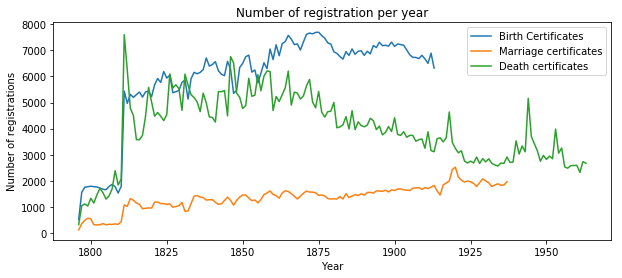
\includegraphics[scale=0.6]{figures/opbouw_registrations.png}
		\label{fig:number_of_registrations}
	\end{center}
\end{figure}
\\

The original documents consists of books with preprinted pages on which an official filled in the specific details of the event. In earlier versions, the entire document were completely handwritten. These books eventually became preprinted book for which only the personal details and details of the event needed to be filled in. An example of a preprinted birth-certificate can be seen in figure \ref{fig:birth_certificate_example}. 



\begin{figure}
	\caption{An example of a birth-certificate. Source: Zeeuws Archief, http://www.archieven.nl}
	\begin{center}
		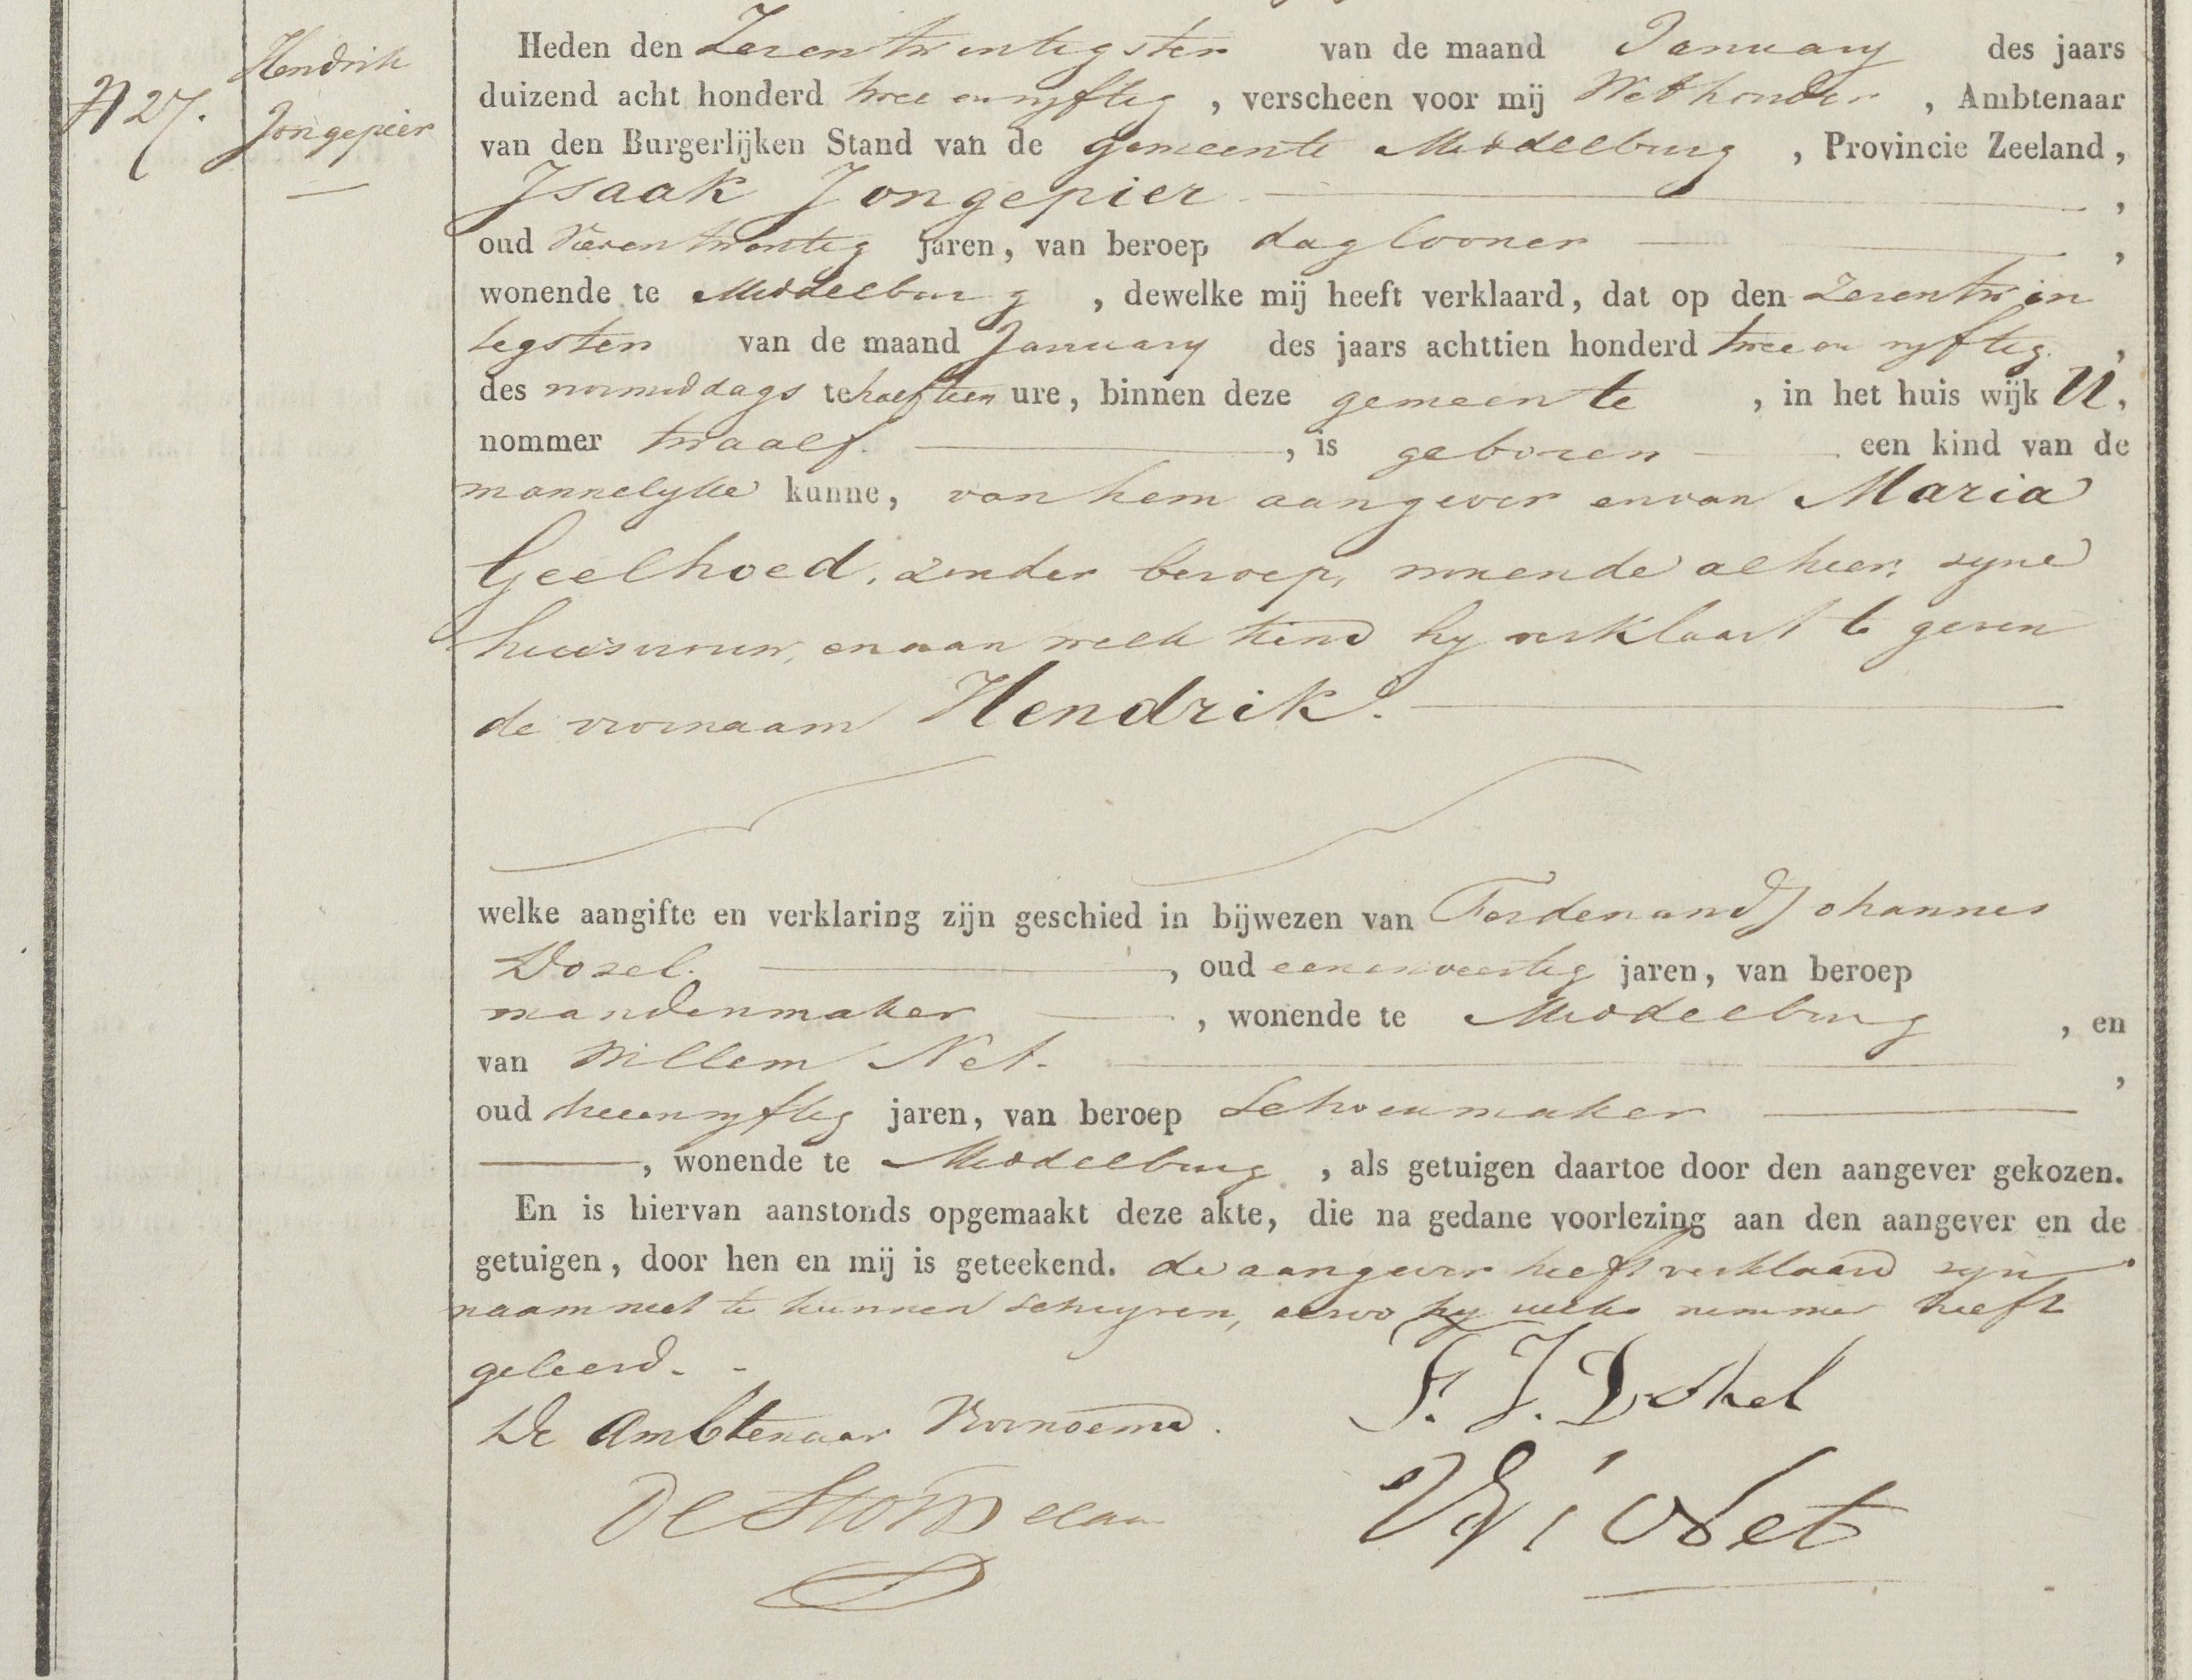
\includegraphics[scale=0.4]{figures/middelburg-gb_1853.jpg}
	\end{center}
	\label{fig:birth_certificate_example}
\end{figure}


The digitalized certificates are stored in the database as the following entities:
\begin{enumerate}
	\item Persons, which contains data concerning the people and events mentioned on a registration, where each record annotates a single person,
	\item Registrations, containing meta-data (such as dates of the registration and the location id),
	\item Locations, containing a mapping from location id to names of locations
\end{enumerate}

The Persons table contains records for each person mentioned in a certificate. The number of persons mentioned on a certificate depends on the type of certificate. On birth-certificates, there are three persons mentioned: child, the mother and the father, where the latter can be absent. Six persons are mentioned on marriage-certificates: the bride and groom, and the mothers and fathers of the bride and groom. On death-certificates at least the deceased and his/her parents are mentioned. In the case that the deceased had a partner, this partner could also be mentioned, but this is not necessarily the case. 
Each 'role' that a person has is also specified (e.g. bride, groom, father of the bride, mother of the groom, etc). The name of each person is split into the first name, surname with, if applicable, a prefix.\\

In table \ref{tab:persons_record_overview_birth}, an example of how a single birth-certificate is stored is shown. For the sake of brevity, only the relevant values are displayed. For each person that was born, at least the day, month and year of the birth has been recorded. The same pattern is also valid for both marriage- and death-certificates, but then the date is stored in mar\_day, mar\_month, mar\_year and their respective death-counterparts, as shown in table \ref{tab:persons_record_overview_marriage} and table \ref{tab:persons_record_overview_death}.\\

Other information that is also recorded in the database include the place of the event and the date. \\
In the next sections, we will ignore most of the meta data and locations of the registrations, and focus only on the names provided on the registrations, and we will use the dates of the registrations.

\begin{landscape}
	\begin{table}
		\centering
		\caption[Overview of a birth-certificate]{An overview of the fields in a birth certificate}
		\begin{tabular}{@{}*2{c}*3{l}*5{c}@{}}
			\toprule
			id\_person & id\_registration & firstnames & prefix & familyname & sex & role & birth\_day & birth\_month & birth\_year \\
			\midrule
			15405 & 5136 & maria cornelia & van & oorsel & f & 1 & 17 & 9 & 1864\\
			15406 & 5136 & willem hendrik & van & oorsel & m & 3 &  &  & \\
			15407 & 5136 & neeltje johanna &  & christiaanse & f & 2 &  &  & \\
			\bottomrule
		\end{tabular}
		\label{tab:persons_record_overview_birth}
	\end{table}
	\begin{table}
		\centering
		\caption[Overview of a marriage-certificate]{An overview of the fields in a marriage certificate}
		\begin{tabular}{@{}*2{c}*3{l}*5{c}@{}}
			\toprule
			id\_person & id\_registration & firstnames & prefix & familyname & sex & role & mar\_day & mar\_month & mar\_year \\
			\midrule
			2095765 & 698592 & cornelis jan &  & dogger & m & 7 & 16 & 8 & 1916\\
			2095766 & 698592 & jacob &  & dogger & m & 9 &  &  & \\
			2095767 & 698592 & pietertje &  & eelman & f & 8 &  &  & \\
			2095768 & 698592 & dina maria & de & rijke & f & 4 & 16 & 8 & 1916\\
			2095769 & 698592 & josua & de & rijke & m & 6 &  &  & \\
			2095770 & 698592 & sara & van de & wege & f & 8 &  &  & \\
			\bottomrule
		\end{tabular}
		\label{tab:persons_record_overview_marriage}
	\end{table}
	\begin{table}
		\centering
		\caption[Overview of a death-certificate]{An overview of the fields in a death certificate}
		\begin{tabular}{@{}*2{c}*3{l}*5{c}@{}}
			\toprule
			id\_person & id\_registration & firstnames & prefix & familyname & sex & role & death\_day & death\_month & death\_year \\
			\midrule
			3258901 & 892601 & izaak &  & lampers & m & 10 & 9 & 8 & 1878\\
			3258901 & 892602 & izaak &  & lampers & m & 3 &  &  & \\
			3258901 & 892603 & catharina &  & dourleijn & f & 2 &  &  & \\
			\bottomrule
		\end{tabular}
		\label{tab:persons_record_overview_death}
	\end{table}
\end{landscape}

\section{Preprocessing}
\subsection{Initial Matching}
The first step is to extract the data that is needed to match the certificates using the method used in \cite{Aspects001}. Since the names of parents are present on each of the certificates, we can extract these names as strings to match.\\

The set of certificates are separated into three sets, based on the nature of the certificates: a set of marriage certificates, a set of birth certificates and a set of death certificates. For each certificate, the first name and family name of the parents are extracted and stored with the certificate id. When multiple names of a person are present for a specific type of name, only the first name is used. For instance: in the case of the first name \textit{bernardus franciscus}, only the name \textit{bernardus} will be used. 
In the case of marriage certificates, two pairs of parents are present on a single certificate (the names of the parents of the bride and groom). These two pairs are both extracted using the role descriptor in the Person table, which indicates the role of the person. The two parent pairs are stored on a seperate line.\\
After this procedure, we have three files that contain the names of the parents mentioned on the registrations. These files will be used as candidate sets when matching the names to the target set.\\

The target set consists of the names of the bride and groom on the marriage certificates. These names are extracted in the same way as the names of the candidate sets by looking at the role of the person. Whenever a person has multiple names, only the first name is used. 
This way, we can couple the birth, marriage and death certificates of the children of the groom and bride to the marriage event of the groom and bride, by matching the names of the groom and bride, and create sets of families: the life events of all the children are coupled to the marriage events of the parents. \\

Table \ref{tab:number_of_registations} shows the number of resulting pairs of parents per set, and table \ref{tab:exerpt_of_target_file} shows the result of the extraction of the names for four of the marriage certificats. The target entries in this table are the groom and bride mentioned on these four registrations, and the entries in the candidate rows are the names of the parents of the groom and bride. \\

\begin{table}
	\centering
	\caption[Number of registration in matching sets]{\label{tab:number_of_registations} The number of parent pairs per candidate set. A candidate set contains the names of the parents mentioned on a registration, while the target set contains the names of the bride and groom on the marriage certificates.}
	\begin{tabular}{lc}
		\toprule
		 & Number of registrations\\
		 \toprule
		 target set (Marriages) & 193,040\\
		 \midrule
		 Birth certificates & 698,199\\
		 Marriage certificates & 386,080\\
		 Death certificates & 665,903\\
		 \bottomrule		 
	\end{tabular}
\end{table}

\begin{table}
	\centering
	\caption[Example of target and candidate files]{\label{tab:exerpt_of_target_file}Exerpts of the target and candidate files, containing the names of the bride and groom on marriage certificates (targets) and the pairs of the parents (candidates)}
	\resizebox{\columnwidth}{!} {
		\begin{tabular}{l*4{c}|l|l*4{c}}
			\toprule
			\multicolumn{5}{c|}{Target entries} && \multicolumn{5}{c}{Candidate entries}\\
			\midrule
			698558 	& cornelis 	& nijssen 		& anna 			& huijssen	 	&& 698558 & jan 		& nijssen 		& johanna 		& pleijte\\
					& 			& 				&	 			& 				&& 698558 & cornelis 	& huijssen 		& elizabeth 	& gouwe\\
			698565 	& adriaan 	& heijnsdijk 	& neeltje 		& hamer 		&& 698565 & geleijn 	& heijnsdijk	& pieternella 	& verpoorte\\
					& 			& 				& 				& 				&& 698565 & cornelis 	& hamer 		& janneke 		& wege\\
			698612 	& adriaan 	& verpoorte 	& pieternella 	& poorter 		&& 698612 & adriaan 	& verpoorte 	& janna 		& hoeve\\
					& 			&  				& 				& 				&& 698612 & michiel 	& pooter 		& pieternella 	& oppeneer\\
			698616 	& aarnoud 	& heynsdijk 	& cornelia 		& bokx 			&& 698616 & jaspert 	& heynsdijk 	& cornelia 		& galle\\
					& 		 	&  				& 				& 				&& 698616 & gilles 		& bokx 			& adriana 		& dieleman\\
			\bottomrule
		\end{tabular}
	}
\end{table}